\documentclass[a4paper, 12 pt]{report}
\usepackage{amssymb}
\usepackage{amsmath}
\usepackage{multirow}
\usepackage{graphicx}
\usepackage{tabularx}
\usepackage{geometry}
\geometry{left=2.5cm,right=2.5cm,top=2.5cm,bottom=2.5cm}
\usepackage{algorithm}  
\usepackage{algorithmic}
\usepackage{tikz}
\usetikzlibrary{shapes.geometric, arrows}



% -------------------------------------------------------------------------------------
% BEGIN DOCUMENT
% -------------------------------------------------------------------------------------
\begin{document}
\title{Drone Design Manual}
\author{Shao Hui z5155945}
\date{}
\maketitle
\pagestyle{empty}
\setcounter{section}{0}
% -------------------------------------------------------------------------------------
% TABLE OF CONTENTS
% -------------------------------------------------------------------------------------
\tableofcontents
\newpage

% -------------------------------------------------------------------------------------
% INTRODUCTION
% -------------------------------------------------------------------------------------
\section{Introduction}
This project simulates a drone searching for a accident scene in a mountain which is presented by a 64$\times$64 matrix.\\
Drone starts searching from possition (0,0), then fly east and searching grids one by one.
Once the drone reaches the boarder of the mountain, it will fly south for 1 meter, then fly to the other direction.
Program keeps the drone suspend above the mountain by 1 meter to make sure every spot can be seen.\\



\newpage
\section{Diagram}
% -------------------------------------------------------------------------------------
%-------------------------
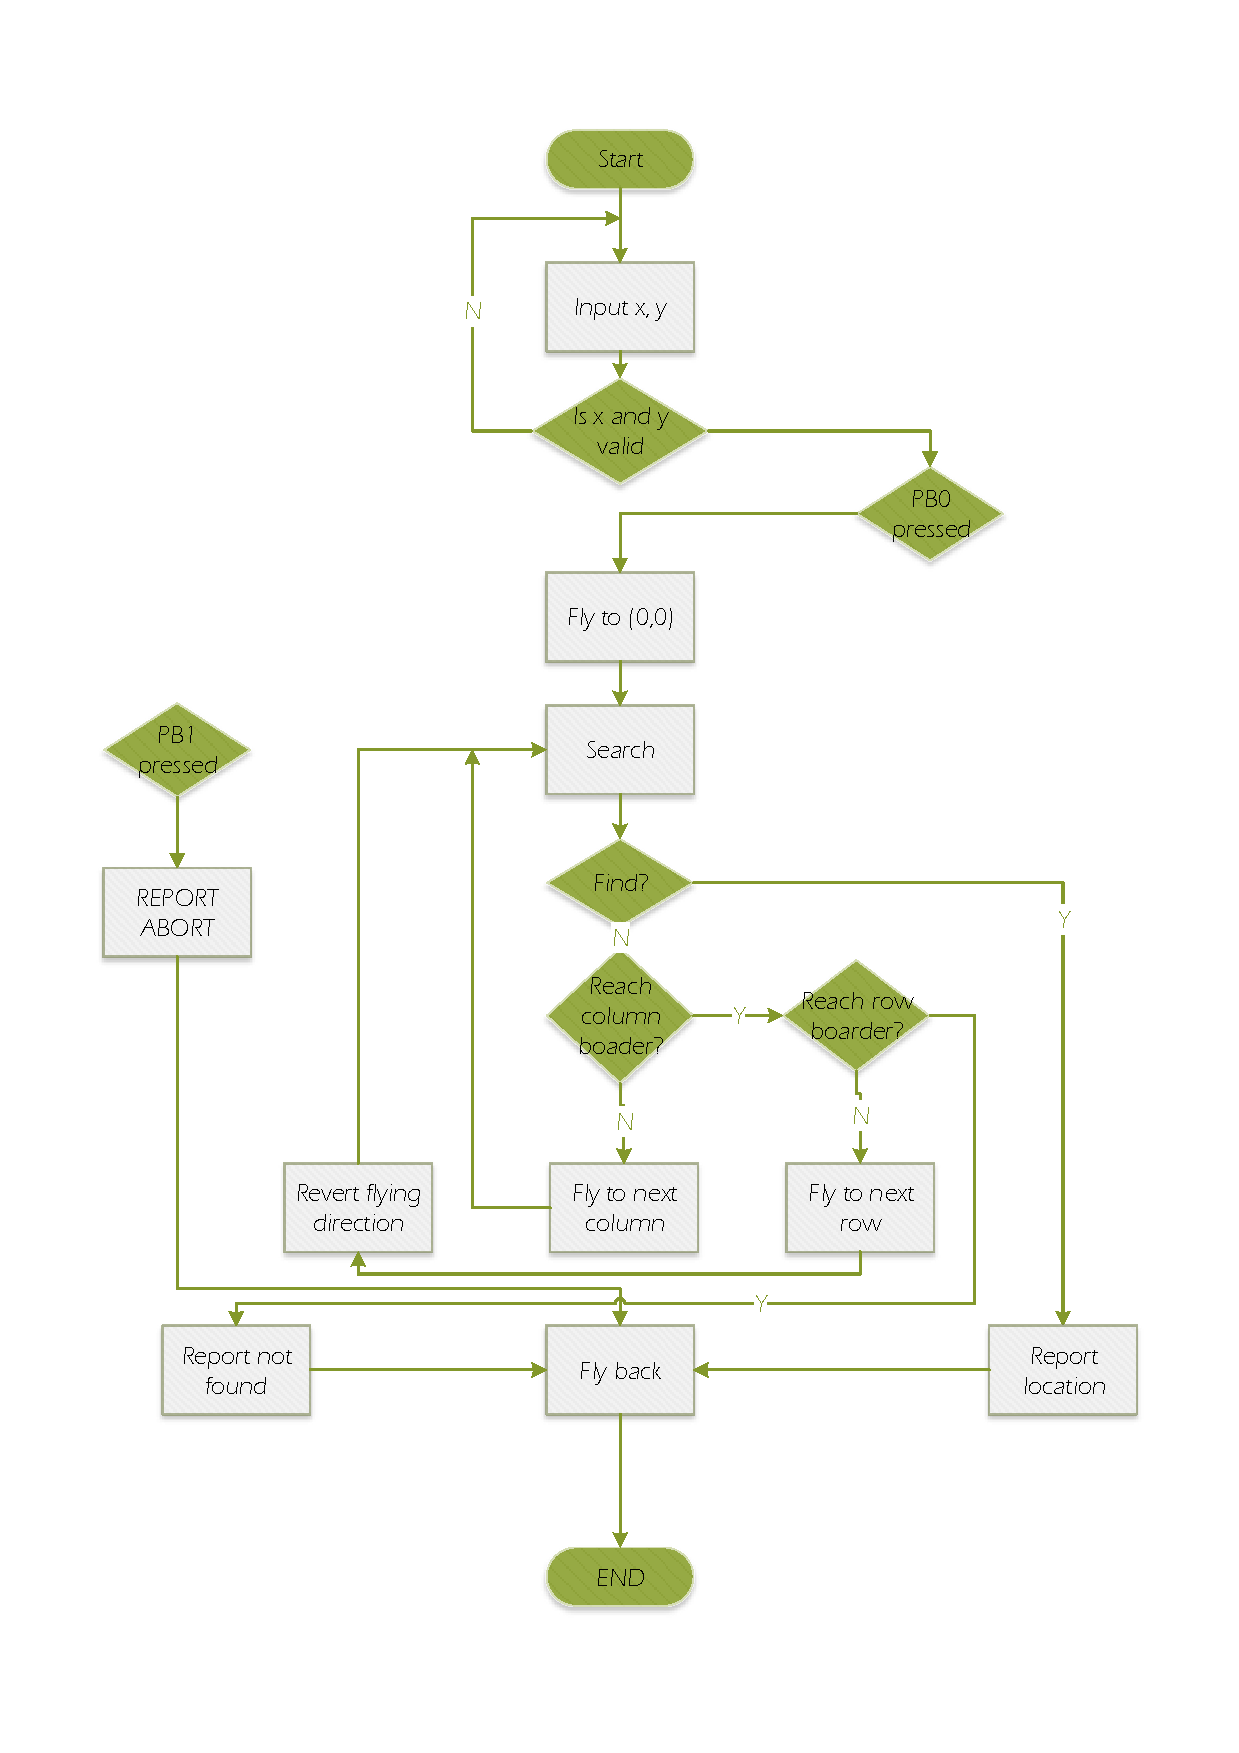
\includegraphics[height = 250mm]{diagram.pdf}


\newpage

% -------------------------------------------------------------------------------------
% Mountain Generator
% -------------------------------------------------------------------------------------
\section{Modules}
\includegraphics[height = 250mm]{tables.pdf}
\newpage
\section{Algorithms}
\begin{algorithm}
    \caption{Fly to next position}
    \label{alg1}
    \begin{algorithmic}[1]
        \STATE try go to next position as direction shows
        \IF{border reached}
            \STATE go south
                \IF{border reached}
                \RETURN -1
                \ENDIF
            \STATE flip direction
        \ENDIF
        \RETURN position height
    \end{algorithmic}
\end{algorithm}
\begin{algorithm}
    \caption{Drone search}
    \label{alg2}
    \begin{algorithmic}[1]
        \STATE read accident position
        \IF {accident scene find}
        \RETURN $true$
        \ELSE
        \RETURN $false$
        \ENDIF
    \end{algorithmic}
\end{algorithm}
\newpage
% -------------------------------------------------------------------------------------
% Control Procedure
% -------------------------------------------------------------------------------------
\section{Data Structure}
\subsection{Mountain}
Mountain is store in program memory as a 2 dimension array of 8bit integer.\\
The index of the array presents the relative position of each 1$\times$1 grid.
The value stored in array presents the height of each position.\\
To get each position's address simply follow such formular.
$$ addr\_position_{x,y} = addr_{Mountain start} + x\times 63 + y$$
\subsection{Accident scene}
Accident scene is stored in data memory as a two 8bit integer, and can be modified by user.\\
Sure we can store accident scene by modify mountain height(eg. plus 128), but store it in the data memory can save it for more general use.
\end{document}
